
\documentclass[10pt,letterpaper]{article}

% =========================================================
% 1. Page Layout & Typography
% =========================================================
\usepackage[left=1in,right=1in,top=1in,bottom=1in]{geometry}
\usepackage[T1]{fontenc}
\usepackage[utf8]{inputenc}
\usepackage{lmodern}
\usepackage{microtype}
\usepackage{url}
% Minimal glyphtounicode placeholder for arXiv/Overleaf

\pdfgentounicode=1

% =========================================================
% 2. Math, Figures & Packages
% =========================================================
\usepackage{amsmath,amssymb}
\usepackage{graphicx}
\usepackage{cite}
\usepackage{indentfirst}
\usepackage{authblk}
\makeatletter
\renewcommand\AB@affilnote[1]{\raisebox{0.35ex}{\scriptsize#1}\hspace{0.08em}}
\makeatother
\usepackage[font=small,labelfont=bf]{caption}
\usepackage[hidelinks]{hyperref}
\usepackage{titlesec}
\usepackage{enumitem}
\usepackage{float}

% =========================================================
% 3. Tables & Color Palette
% =========================================================
\usepackage[table,xcdraw,dvipsnames]{xcolor}
\usepackage{booktabs}
\usepackage{multirow}
\usepackage{pifont}
\usepackage{textcomp}
\usepackage{array}

\definecolor{npsgreen}{HTML}{E1F1EC}
\definecolor{npsred}{HTML}{FEECDD}
\definecolor{cvprblue}{HTML}{DEEBF7}
\definecolor{icmlred}{HTML}{E58579}
\definecolor{cvprgreen}{HTML}{BBDBA6}
\definecolor{cvprorange}{HTML}{F4B183}
\definecolor{lightblue}{HTML}{DCEAF7}
\definecolor{lightgreen}{HTML}{E8F3E1}
\definecolor{lightorange}{HTML}{F9E7D2}
\definecolor{graybg}{gray}{0.95}

\newcommand{\cmark}{\textcolor{ForestGreen}{\ding{51}}}
\newcommand{\xmark}{\textcolor{BrickRed}{\ding{55}}}
\newcommand{\approxw}[1]{\ensuremath{\sim #1\,\mathrm{W}}}

% =========================================================
% 4. TikZ Drawing Library
% =========================================================
\usepackage{tikz}
\usetikzlibrary{shapes.geometric, arrows.meta, positioning, fit, backgrounds, shadows, calc}

\tikzset{
    basebox/.style={rectangle, draw=gray!60, thick, rounded corners=3pt, align=center, fill=white, font=\small, drop shadow={opacity=0.05}},
    frontbox/.style={basebox, fill=cvprblue!45, minimum height=1cm},
    agentbox/.style={basebox, fill=npsgreen!80, minimum height=1cm},
    toolbox/.style={basebox, fill=cvprorange!45, minimum height=1cm},
    edgebox/.style={basebox, fill=lightgreen!75, minimum height=1cm},
    note/.style={basebox, fill=gray!8, font=\scriptsize},
    arrow/.style={->, >=Stealth, thick, draw=gray!80},
    dasharrow/.style={->, >=Stealth, dashed, thick, draw=gray!80}
}

\setlength{\parindent}{1.2em}
\setlength{\parskip}{0pt}
\setlength{\affilsep}{0.2em}
\renewcommand{\abstractname}{ABSTRACT}
\renewcommand{\refname}{REFERENCES}
\renewcommand\Authfont{\fontsize{12}{15}\selectfont}
\renewcommand\Affilfont{\fontsize{10}{14}\selectfont\raggedright}
\renewcommand{\thesection}{\Roman{section}}
\setcounter{secnumdepth}{1}
\titleformat{\section}{\normalfont\bfseries\centering}{\thesection.}{0.6em}{\MakeUppercase}
\titleformat{name=\section,numberless}{\normalfont\bfseries\centering}{}{0pt}{\MakeUppercase}
\titleformat{\subsection}{\normalfont\bfseries}{}{0pt}{}
\titlespacing*{\section}{0pt}{1.25\baselineskip}{0.75\baselineskip}
\titlespacing*{\subsection}{0pt}{0.9\baselineskip}{0.45\baselineskip}
\captionsetup{justification=raggedright,singlelinecheck=false}
\setlist[enumerate]{leftmargin=1.5em,itemsep=0.25em,topsep=0.35em}

% =========================================================
% TITLE & AUTHORS
% =========================================================
\title{SAT-Edge-Agent: Hardware-in-the-Loop Edge-Agent Orchestration\\
for Onboard Satellite Intelligence}

\author{}
\date{}
\newcommand{\affline}[2]{%
  \noindent\hangindent=1.5em\hangafter=1%
  \makebox[1.5em][r]{\textsuperscript{#1}}#2\par
}

\begin{document}
\maketitle
\vspace{-4.4em}
\begin{center}
{\fontsize{12}{15}\selectfont
Longji He$^{1,2}$ and Jeto Xu$^{1}$}
\end{center}
\vspace{0.55em}
{\fontsize{10}{14}\selectfont
\affline{1}{OgCloud Limited, Guangzhou, GD, China, \texttt{keith@ogcloud.com}}
\affline{2}{College of Engineering, The Pennsylvania State University, University Park, PA, USA}
}
\vspace{0.85em}

\begin{abstract}

Onboard satellite intelligence requires a task layer that turns mission intent into local tool calls, coordinates perception and language services, exposes progress, and returns structured artifacts under communication and power constraints. We present SAT-Edge-Agent, a hardware-in-the-loop (HIL) edge-agent system deployed on a commercial off-the-shelf (COTS), ARM-based heterogeneous edge system-on-chip (SoC). It integrates a React/Vite operator workspace, a FastAPI agent backend built with LangChain/LangGraph components, a local OpenAI-compatible language-model service, and a project-internal YOLO-style oriented-object-detection endpoint that propagates FAIR1M-provided geographic metadata into structured results. We evaluate one fixed FAIR1M image and one fixed serial two-image pair over 20 attempts each; both workloads achieved 20/20 observed completion. Mean full-Agent latency was 29.353 s and 60.937 s, with empirical nearest-rank P95 values of 31.166 s and 66.882 s. Mean cumulative detector time was 861.386 ms and 1510.920 ms, representing 2.93\% and 2.48\% of mean full-Agent latency. A separate profiler set shows that most user-visible time lies outside detector execution, across Agent orchestration and local response formation before and after the first visible token. The two per-workload mean CPU values span 20.5--20.8\%. A devfreq/sysfs NPU-load field sampled every 200 ms across the full request remained at 100\%; because the detector and local language service share the accelerator, this is not detector-only occupancy or calibrated utilization. A sanitized request-level evidence package reproduces the reported statistics and provides redacted JSON plus normalized success and partial-failure SSE examples. A separate earlier plug-meter pilot is retained only as unsynchronized board-level context. These results establish repeated fixed-workload HIL evidence and a reproducibility boundary for satellite edge-agent orchestration, not detector accuracy, a new geolocation algorithm, calibrated energy efficiency, or flight validation.

\textbf{Keywords:} satellite edge computing, hardware-in-the-loop, onboard intelligence, edge agent, COTS edge SoC, local LLM service, remote sensing, oriented object detection, FAIR1M, power-aware edge AI
\end{abstract}

\section{Introduction}

Low-Earth-orbit Earth-observation missions increasingly require interpretation to move closer to the sensor. A satellite that only stores and forwards raw imagery remains dependent on communication windows, downlink bandwidth, ground-side inference, and manual task interpretation. Onboard AI changes this pattern by allowing the spacecraft or payload computer to filter low-value scenes, identify high-value events, and return compact mission products before the full image archive is downlinked \cite{phisat1,cloudscout,ravaen}. Recent orbital-edge and satellite-edge studies make the same systems point in a broader form: sensing volume, contact intermittency, latency, and energy constraints make purely ground-side processing an increasingly poor default for time-sensitive missions \cite{oec_asplos,satedge_tcom,ai_onboard_survey}.

The next step is not merely to place one detector on a board. A useful onboard-intelligence payload needs a task layer. It must receive user or mission intent, decide which local tool should be invoked, pass data to a vision service, optionally coordinate local language-model reasoning, stream intermediate state, and return structured results that a ground operator or downstream machine system can consume. This is especially relevant as satellite-edge artificial intelligence begins to consider large models and microservice-style inference at the satellite edge \cite{satellite_edge_large_models}. In this setting, the spacecraft is no longer only a remote sensor. It becomes a constrained, power-aware edge computer that produces mission artifacts and sends back the result when that is more valuable than sending every raw frame.

SAT-Edge-Agent addresses this systems problem. The project is built around a HIL edge setting in which a low-power COTS ARM-based heterogeneous edge-SoC platform hosts local inference services and exposes them through an agent workflow. The vision service returns oriented object detections and FAIR1M metadata-backed geographic target fields from remote-sensing images \cite{fair1m}. The local LLM service provides an OpenAI-compatible interface. The agent backend coordinates tool invocation and streams response events to a browser-based workspace.

The key contribution is not a new YOLO architecture, and the present paper is not a flight demonstration. The paper instead asks a narrower implementation question: how can satellite edge inference be organized as an end-to-end, reproducible agent workflow on a low-power edge SoC, and what evidence can a HIL deployment provide without overstating the current artifact? This framing follows a systems-paper logic. A detector paper would need a rigorous accuracy comparison, training protocol, model release, and benchmark evaluation. A HIL system paper must instead show that components can be integrated, deployed, invoked, observed, measured within a stated boundary, and reproduced by other users to the extent permitted by data and model licenses.

Power awareness remains part of the systems boundary, but the current evidence is intentionally secondary. A separate 2026-07-03 plug-meter pilot is retained in Appendix~\ref{app:artifacts} as board-level context. It was not recorded concurrently with the repeated 2026-07-13 FAIR1M latency experiment and is therefore not used to claim calibrated power, energy per request, or spacecraft energy efficiency.

The paper makes four contributions:
\begin{enumerate}
    \item It presents SAT-Edge-Agent as an end-to-end HIL edge-agent architecture that combines a browser workspace, FastAPI agent backend, local LLM service, and a project-internal YOLO-style OBB detector endpoint on a COTS ARM-based heterogeneous edge SoC.
    \item It documents a reproducibility boundary that separates public source code, service contracts, runtime metadata, dataset-license constraints, private model weights, and internal laboratory infrastructure.
    \item It demonstrates how a vision detector can be used as an agent tool to produce structured remote-sensing mission artifacts with class labels, confidence scores, oriented polygons, pixel centers, and FAIR1M metadata-backed geographic target fields.
    \item It reports repeated fixed-workload full-Agent and YOLO-tool latency, visible-response timing, observed completion, and CPU/NPU telemetry for single-image and serial two-image FAIR1M workflows, while keeping an earlier plug-meter power pilot explicitly separate from the repeated latency evidence.
\end{enumerate}

\section{Related Work}

\subsection{Onboard Autonomy and Satellite AI}

Autonomous spacecraft and onboard sciencecraft systems show that spacecraft can detect events, plan responses, and reduce dependence on continuous ground control. EO-1-style autonomous science operations and onboard classifiers for science-event detection are important precedents because they demonstrate that onboard software can identify high-value observations and alter what is returned to the ground \cite{eo1_sciencecraft,onboard_classifiers}. Recent Earth-observation AI missions such as Phi-Sat-1 and CloudScout show that neural-network inference can be executed onboard satellite payloads for tasks such as cloud filtering and downlink selection \cite{phisat1,cloudscout}. RaVAEn and later onboard-training work further show that compact learned representations can support onboard change detection, inference, and limited training under satellite hardware constraints \cite{ravaen,fast_onboard_training}. These missions motivate SAT-Edge-Agent's direction, but the present paper occupies a different layer. It does not only ask whether a neural model can run onboard; it asks how edge inference can be wrapped inside a mission-facing agent workflow with a reproducible HIL boundary.

\subsection{Satellite Edge Computing and COTS Hardware}

Satellite edge computing treats orbital and near-orbital nodes as compute systems close to the sensor \cite{oec_asplos,satedge_tcom}. This perspective is useful for missions where raw data volume, latency, ground-station visibility, and energy constrain operational value. Recent surveys and workshop reports also emphasize the practical obstacles: restricted power, memory, storage, radiation environment, incomplete datasets, and the need to benchmark AI workloads on realistic embedded processors \cite{ai_onboard_survey,gardill_space_edge}. Broader heterogeneous edge-platform benchmarking further shows that CPU, GPU, and NPU advantages depend on the workload and metric, so processor-level speedup values should not be transferred across unlike tasks \cite{edge_ai_platform_benchmark}. The edge-SoC evidence in this paper should be read in that HIL sense. It supports a ground-based edge-payload prototype and a power-aware software stack, not a radiation-qualified flight-computer claim.

\subsection{Agent Orchestration for Edge AI}

Tool-using LLM systems provide a convenient abstraction for workflows that must decide when to call detectors, when to summarize results, and how to stream intermediate state. ReAct studies the interleaving of reasoning traces and actions, Toolformer studies language models that learn to call external APIs, and recent agent surveys organize LLM-based autonomous agents around planning, memory, tool use, and evaluation \cite{react,toolformer,llm_agents_survey}. A recent Earth-observation preprint also explores hierarchical multi-agent routing for onboard crisis-response analysis on an engineering edge platform \cite{onboard_multiagent_eo}. SAT-Edge-Agent uses this agentic abstraction in a bounded engineering way. The local LLM is not claimed to be a fully autonomous mission planner in this version. It is a mission-facing orchestration layer that turns local inference services into structured edge workflows.

\subsection{Remote-Sensing OBB Detection and FAIR1M}

Remote-sensing imagery often contains rotated, dense, and fine-grained targets. DOTA helped establish oriented object detection in aerial imagery by annotating objects with arbitrary quadrilaterals, while FAIR1M provides high-resolution imagery, oriented bounding boxes, fine-grained categories, and geographic metadata suitable for aircraft, ship, and vehicle analysis \cite{dota,fair1m}. Remote-sensing detection reviews and OBB surveys further show why orientation-aware target representations are important in optical remote-sensing imagery \cite{rsod_review,obb_survey}. SAT-Edge-Agent uses this style of data because the output artifacts are naturally mission-oriented: classes, confidence, oriented polygons, and dataset-provided geographic fields can be serialized into structured task results. In this paper, FAIR1M and the YOLO26-labeled service support the agent workflow as a vision tool. They are not used to claim a new state-of-the-art detector or a new geolocation algorithm.

\subsection{Comparative Positioning and System-Level Efficiency}
\label{sec:comparative_positioning}

The measured value of SAT-Edge-Agent should be compared at the correct system layer. Existing onboard-AI work provides strong evidence that neural models can run close to the sensor: Phi-Sat-1 and CloudScout demonstrate cloud filtering for downlink selection, RaVAEn demonstrates compact representation learning and onboard model execution, and Myriad/Snapdragon benchmarks show that COTS or COTS-derived edge processors can provide substantial model-dependent acceleration under space-relevant test conditions \cite{phisat1,cloudscout,ravaen,fast_onboard_training,edge_processor_benchmark}. These studies are essential precedents, but their metrics are mostly model-level metrics such as classifier accuracy, encoding time, inference time, quantization discrepancy, power, or energy per inference. They are not direct baselines for an Agent workflow that combines a detector endpoint, local language-model service, streamed task state, and structured mission-result generation.

\begin{table}[htbp]
\centering
\small
\renewcommand{\arraystretch}{1.12}
\begin{tabular}{p{0.19\linewidth}p{0.24\linewidth}p{0.24\linewidth}p{0.24\linewidth}}
\toprule
\textbf{Reference layer} & \textbf{Reported value type} & \textbf{What it supports} & \textbf{Comparison boundary} \\
\midrule
Phi-Sat-1 / CloudScout & Onboard cloud-filtering accuracy, embedded inference, and downlink-selection motivation & Onboard AI can remove or deprioritize low-value Earth-observation data before downlink & Different task and output artifact; not a direct latency or accuracy baseline for OBB Agent workflows \\
RaVAEn onboard model execution & Tile-level representation encoding and onboard model execution/training evidence & Compact learned representations can be executed near the sensor and used for downstream prioritization & Different model, data unit, and mission product; useful for context, not a speedup denominator \\
Myriad/Snapdragon benchmark & Processor-dependent inference time, quantization discrepancy, and energy/power measurement methodology & Edge-processor benchmarking must report workload, hardware path, transfer overhead, and metric scope & Supports measurement discipline; does not benchmark SAT-Edge-Agent's FastAPI/LLM/YOLO workflow directly \\
SAT-Edge-Agent HIL evidence & Repeated fixed-workload YOLO-tool and full-Agent timing, CPU/NPU telemetry, structured partial-failure behavior, and metadata-backed artifacts & A mission-facing Agent workflow can coordinate local tools and return structured remote-sensing results on a COTS ARM-based heterogeneous edge SoC & Current evidence covers two fixed HIL workloads; it should not be generalized to broad mission distributions, flight performance, or calibrated energy efficiency \\
\bottomrule
\end{tabular}
\caption{Comparative positioning of SAT-Edge-Agent against measured onboard-AI and edge-processor studies. The table separates model-level performance evidence from workflow-level HIL evidence so that the paper does not imply an invalid speedup comparison.}
\label{tab:comparative_positioning}
\end{table}

This distinction changes the efficiency claim. SAT-Edge-Agent should not be described as universally faster than prior onboard-AI systems, because the tasks, processors, data units, and output contracts differ. Its present efficiency contribution is system-level: a YOLO-style OBB endpoint is embedded inside a mission-facing workflow that also performs Agent routing, annotated-result rendering, local response synthesis, SSE-visible state streaming, and structured artifact generation. In the repeated HIL runs, detector time and full-Agent time are intentionally reported separately. The single-image detector call averaged 0.861 s, while the cumulative serial two-image detector stage averaged 1.511 s; these values represented only about 2--3\% of the corresponding full-Agent means. The evidence therefore isolates a clear optimization boundary without assigning every remaining millisecond to the language model alone. Payload-size and transfer-time benefits of returning structured results instead of raw images are complementary and are evaluated separately in the public downlink-payload experiment.

\section{System Architecture}
\label{sec:architecture}

\subsection{Architecture Overview}

SAT-Edge-Agent consists of four active runtime layers and one evidence layer: a browser-based operator workspace, a FastAPI agent backend, a project-internal YOLO-style OBB detector service, a local LLM service, and an artifact boundary that records the runtime and service state. Table~\ref{tab:system_layers} summarizes the division of responsibility.

\begin{table}[htbp]
\centering
\renewcommand{\arraystretch}{1.16}
\setlength{\tabcolsep}{4pt}
\caption{SAT-Edge-Agent system layers. The detector and LLM are treated as tools inside the agent workflow, not as the paper's standalone algorithmic contributions.}
\label{tab:system_layers}
\begin{tabular}{p{0.22\linewidth}p{0.28\linewidth}p{0.40\linewidth}}
\toprule
\rowcolor{gray!12}
\textbf{Layer} & \textbf{Component} & \textbf{Role} \\
\midrule
Operator workspace & React/Vite frontend & Browser interaction and streamed agent result display. \\
\rowcolor{graybg}
Agent service & FastAPI with LangChain/LangGraph components & Prompt handling, tool invocation, state/checkpoint support, and SSE streaming. \\
Vision tool & YOLO-style OBB endpoint & Oriented remote-sensing detection and FAIR1M metadata-backed geographic target fields. \\
\rowcolor{graybg}
Reasoning service & Local OpenAI-compatible LLM endpoint & Local language-model response and mission-summary generation. \\
Evidence layer & Repository artifacts and sanitized runtime records & Reproducibility boundary, service contracts, release notes, and unsupported-claim guardrails. \\
\bottomrule
\end{tabular}
\end{table}

\begin{figure*}[t]
\centering
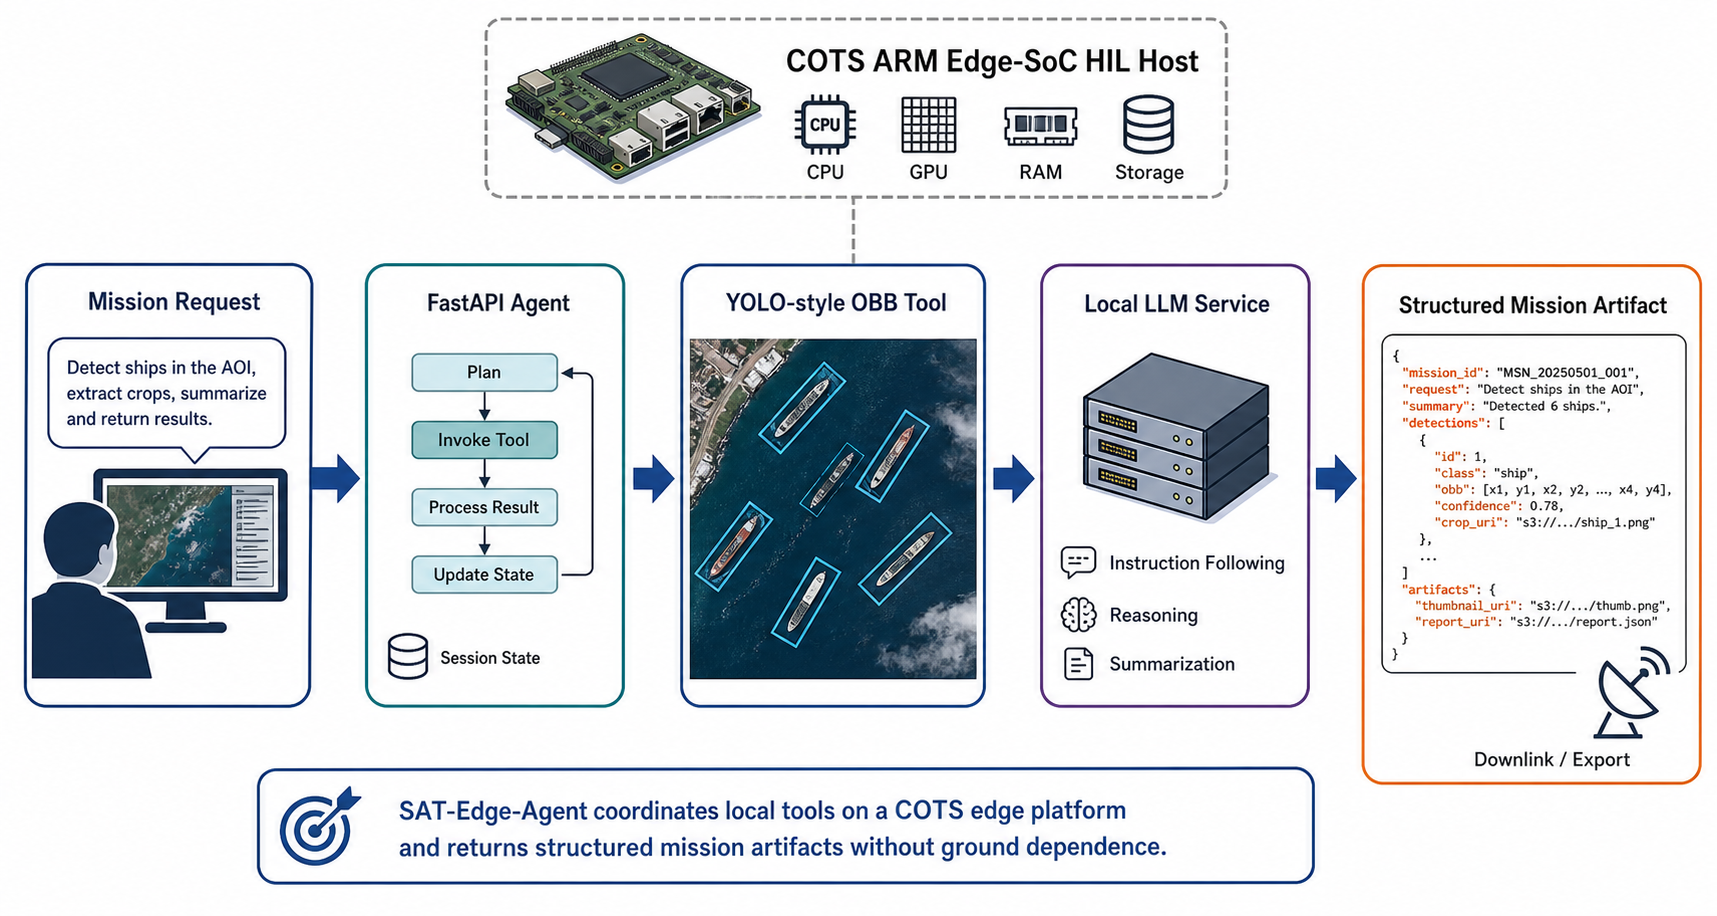
\includegraphics[width=0.98\textwidth]{figures/fig1_system_overview.png}
\caption{SAT-Edge-Agent system overview. A mission request is routed through the FastAPI Agent, which invokes a YOLO-style OBB tool and a local LLM service to return structured mission artifacts from the HIL edge host.}
\label{fig:architecture}
\end{figure*}


\subsection{Hardware-in-the-Loop Boundary}

The HIL boundary in this paper is the edge host and its local services. The recorded runtime snapshot identifies the host as an aarch64 Debian 11 environment running on a COTS ARM-based heterogeneous edge-SoC board. The public manuscript uses sanitized host labels such as \texttt{<edge-host>} and does not expose private IP addresses or access methods. The claim is therefore that SAT-Edge-Agent has been integrated and observed on a COTS ARM-based heterogeneous edge-SoC environment with local detection and language-model services. It is not a claim that the system has been flight-validated or qualified for the space radiation environment.

\subsection{End-to-End Execution Path}

The end-to-end path is intentionally simple and reproducible. A mission request enters through the browser workspace, the FastAPI backend constructs an agent state, the backend invokes the detection tool when an image-grounded answer is required, the detector returns OBB detections with metadata-backed geographic target fields, and the local LLM service generates a compact mission-facing response. The frontend receives server-sent events (SSEs) so that the operator can observe the tool call rather than only the final text. This path is useful for onboard-style payloads because it turns raw sensor output into a structured mission product before downlink.

\subsection{Service Interfaces}

The detection service exposes \texttt{POST /v1/detect}, \texttt{GET /v1/health}, and \texttt{GET /v1/model/status}. The evidence package records a healthy endpoint response and a loaded project-internal OBB weight, image size 1024, object threshold 0.25, and non-maximum-suppression threshold 0.45. The private weight filename is withheld. In this manuscript, YOLO26 is a project-internal service label for a YOLO-style OBB endpoint, not a new public detector family or a standardized YOLO release. These records support service availability and configuration, not detector accuracy. The local LLM service is exposed through an OpenAI-compatible endpoint so that the orchestration layer can remain stable even when the underlying model implementation changes. Model-specific capability tests remain outside the public reproduction claim because their configurations and task boundaries differ from the repeated HIL workflow reported here.

\section{Agent Workflow and Tool Orchestration}
\label{sec:workflow}

\subsection{Workflow Concept}

The agent workflow begins with a user or mission request that references one or more remote-sensing images. The backend determines whether detection is required, invokes the appropriate vision tool, receives structured detections, and produces a concise natural-language interpretation. The frontend receives state through SSEs and can display both text and tool artifacts.

The intended event lifecycle is \texttt{start} $\rightarrow$ \texttt{tool} $\rightarrow$ \texttt{token} $\rightarrow$ \texttt{done}, with structured error fields for failed tool calls or invalid input. The current code and logs support SSE streaming and successful \texttt{/api/v1/chat/stream} calls. The public HIL artifact package includes normalized success and serial-batch partial-failure transcripts with request identifiers, runtime paths, base64 images, private labels, and operator text removed.

\begin{figure*}[t]
\centering
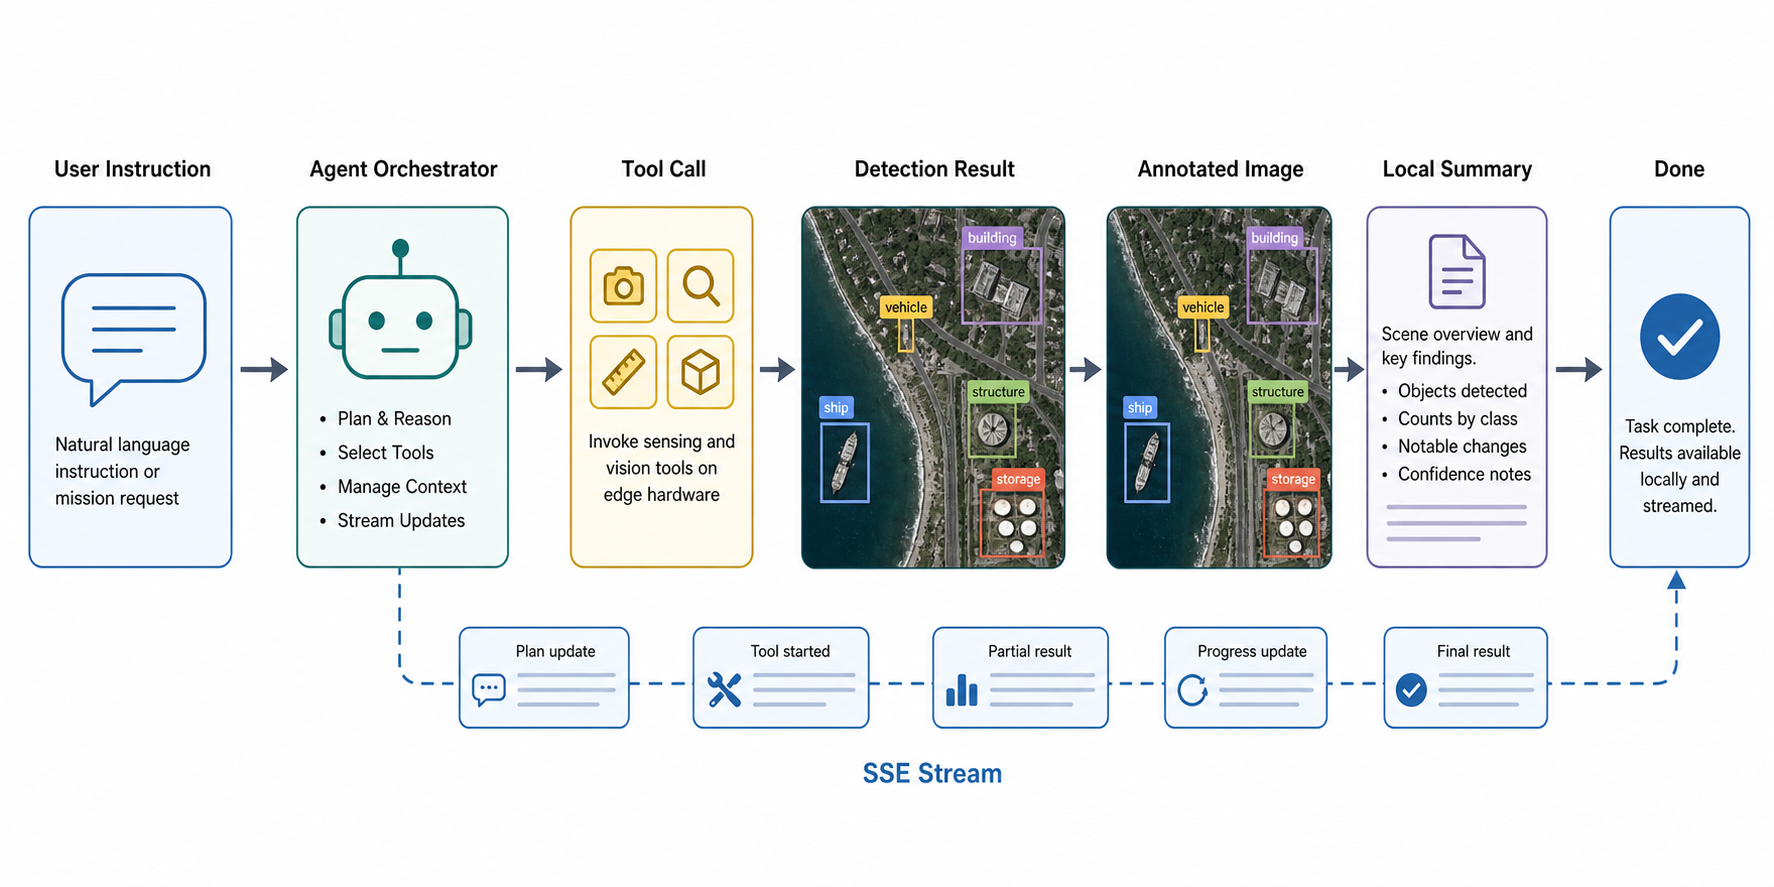
\includegraphics[width=0.98\textwidth]{figures/fig2_hil_workflow.png}
\caption{HIL Agent workflow. The backend receives a user instruction, selects and invokes local tools, converts detections into annotated artifacts and a local summary, and streams intermediate events to the operator interface through SSE.}
\label{fig:workflow}
\end{figure*}


\subsection{Single-Image Analysis}

In the single-image workflow, the agent calls the detector once and receives a structured response containing image metadata, target detections, confidence scores, OBB polygons, pixel centers, and metadata-backed geographic centers. The agent then summarizes what was detected and whether geographic target fields are present. The representative case in the evidence package reports:
\begin{quote}
\texttt{detections=7; classes=A220:2, other-airplane:5; geo\_targets=7; total\_ms=846.646}
\end{quote}
This supports the claim that the system can produce metadata-backed structured mission artifacts from a FAIR1M-style image. The same fixed image is used by the repeated single-image timing protocol in Section~\ref{sec:results}; the representative response illustrates the output schema, whereas the 20-run experiment supports timing and repeatability claims. A compact redacted JSON record is shown with the service-contract evidence, and the complete sanitized example is included in the public artifact package.

\subsection{Failure Handling}

The evidence package includes a deliberately invalid upload. The endpoint returns a structured unsupported-media-type error with the message \texttt{Only jpg/png are supported}, and the service log includes a corresponding \texttt{415 Unsupported Media Type} record. A separate profiler-enabled serial batch exercised a missing second-image path. The tool returned \texttt{images\_count=2}, \texttt{success\_count=1}, and \texttt{failure\_count=1}, preserved a per-image error field, streamed a final response, and reached the SSE \texttt{done} event. Identifiers and runtime paths are omitted from the manuscript. These cases support structured invalid-input and partial-batch reporting, but they do not establish timeout recovery, retries, watchdog behavior, or service-restart correctness.

\subsection{Metadata-Backed Detection Artifacts}

The successful detection example includes request identifier, image file name, width, height, center geographic coordinates, per-target class ID and class name, confidence score, oriented polygon coordinates, pixel center, and geographic center. These geographic fields are not presented as a new geolocation algorithm. In the current evidence package, they are parsed from FAIR1M-style dataset metadata associated with the sample images and objects. When associated metadata are unavailable, the system treats geographic fields as unavailable rather than synthesizing coordinates; no sensor-model or map-registration fallback is implemented. The paper therefore claims metadata propagation and serialization into mission records, not independently validated absolute geolocation accuracy.

For \texttt{train\_\_t\_10144.jpg}, the detection output reports seven targets. Two are classified as \texttt{A220}, and five are classified as \texttt{other-airplane}. Each target contains a geographic center field, allowing the system to return metadata-backed target locations rather than only image-space boxes. This result is a qualitative system-output example. It is not an accuracy benchmark or a geolocation-error benchmark.


\section{Experimental Setup and Evidence}
\label{sec:results}

\subsection{Edge Runtime Snapshot}

Table~\ref{tab:runtime_snapshot} summarizes the HIL edge runtime snapshot used by the current manuscript. The table supports the setup description and should not be interpreted as a space-grade hardware qualification.

\begin{table}[htbp]
\centering
\renewcommand{\arraystretch}{1.16}
\setlength{\tabcolsep}{4pt}
\caption{HIL edge runtime snapshot recorded for the SAT-Edge-Agent evidence package. Private hostnames and paths are sanitized.}
\label{tab:runtime_snapshot}
\begin{tabular}{p{0.30\linewidth}p{0.55\linewidth}}
\toprule
\rowcolor{gray!12}
\textbf{Item} & \textbf{Evidence value} \\
\midrule
Operating system & Debian GNU/Linux 11 (bullseye) \\
\rowcolor{graybg}
Kernel/architecture & Linux 6.1.115, aarch64 \\
Board model & COTS ARM-based heterogeneous edge-SoC board (exact vendor model retained in internal evidence) \\
\rowcolor{graybg}
CPU and memory & 8 Cortex-A55 cores, max 2304 MHz; 31 GiB memory \\
Python runtime & Python 3.13.12 \\
\rowcolor{graybg}
Key packages & requests 2.32.5; FastAPI 0.136.1; Uvicorn 0.46.0; Pydantic 2.13.3; NumPy 2.4.4 \\
Paper branch & \texttt{dev/new-yolo-tool} \\
\bottomrule
\end{tabular}
\end{table}

\subsection{Service-Contract Evidence}

The YOLO-style service evidence records a Uvicorn startup for \texttt{obb\_geo\_api\_server:app} with host \texttt{0.0.0.0} and port \texttt{8003}. The service was observed with a loaded project-internal OBB weight, image size 1024, object threshold 0.25, and NMS threshold 0.45. The exact private weight filename is retained only in internal evidence. Logs show multiple \texttt{POST /v1/detect 200 OK} entries and a deliberate \texttt{415 Unsupported Media Type} failure case. The label YOLO26 is used for this project service and should not be read as a new public detector family.

\begin{table}[htbp]
\centering
\renewcommand{\arraystretch}{1.16}
\setlength{\tabcolsep}{4pt}
\caption{Service-contract evidence for the YOLO OBB tool. These checks support API availability and structured behavior, not detector accuracy.}
\label{tab:service_evidence}
\begin{tabular}{p{0.30\linewidth}p{0.28\linewidth}p{0.30\linewidth}}
\toprule
\rowcolor{gray!12}
\textbf{Evidence item} & \textbf{Observed value} & \textbf{Claim supported} \\
\midrule
Health endpoint & \texttt{status=ok}, version 1.0.0 & Service availability \\
\rowcolor{graybg}
Model status & \texttt{loaded=true}, image size 1024 & Model-loaded service state \\
Success case & Seven detections with metadata-backed geographic fields & Structured output schema \\
\rowcolor{graybg}
Invalid upload & \texttt{UNSUPPORTED\_\allowbreak MEDIA\_\allowbreak TYPE}, HTTP 415 & Structured failure path \\
Partial serial batch & 1/2 images successful; final SSE \texttt{done} emitted & Structured partial-result path \\
\bottomrule
\end{tabular}
\end{table}

The public package preserves the exact field names while removing the request identifier and base64 image. The following compact record shows one of seven detections; coordinates are rounded for presentation.

\begin{small}
\begin{verbatim}
{
  "image": {"file_name": "train__t_10144.jpg",
            "width": 1000, "height": 1000},
  "detections_count": 7,
  "detections": [{
    "class_name": "A220", "confidence": 0.968452,
    "polygon": [[598.936,136.701],[619.303,91.140],
                [581.040,74.035],[560.673,119.596]],
    "pixel_center": [589.988,105.368],
    "geo_center": [118.121802,24.539276]
  }],
  "perf": {"total_ms": 846.646}, "geo_status": "ok"
}
\end{verbatim}
\end{small}

\subsection{Metadata-Backed Output Evidence}

The representative FAIR1M case returns seven detections with metadata-backed geographic target fields. The output includes aircraft classes, confidence values, OBB polygons, pixel centers, and geographic centers parsed from FAIR1M-style sample metadata. This supports the claim that the system can serialize detection outputs into mission-facing records. It does not support an accuracy benchmark, SOTA detector claim, or independently validated geolocation-error claim.

\subsection{Repeated Fixed-Workload HIL Protocol}

The primary performance evidence was collected on 2026-07-13 using two fixed FAIR1M workloads. The single-image workload repeatedly uses \texttt{train\_\_t\_10144.jpg}; the serial workload uses that image followed by \texttt{train\_\_t\_10175.jpg}. Warm-up requests were excluded, and the two-image workload invokes the images serially rather than concurrently. Each workload contains 20 measured attempts. Full-Agent latency starts when the Agent receives \texttt{/api/v1/chat/stream} and ends when the SSE stream emits \texttt{done}; it includes Agent routing, detector invocation, result handling, annotated-output production, local response formation, and SSE delivery. YOLO-tool latency is the detector-stage duration reported by the vision tool. CPU and NPU fields were sampled over the full-Agent window.

The resource sampler queried CPU counters and a devfreq/sysfs NPU load/frequency field at 200-ms intervals. The NPU field spans the complete request and is shared by accelerator consumers, including the detector and local language service. Consequently, a sampled value of 100\% is a coarse shared-accelerator software field; it is not detector-only occupancy, per-service attribution, or a calibrated utilization measurement.

\begin{table}[htbp]
\centering
\small
\renewcommand{\arraystretch}{1.14}
\setlength{\tabcolsep}{3.5pt}
\caption{Fixed-workload protocol for the repeated HIL experiment. The sample counts characterize repeatability for these two workloads, not a FAIR1M-wide latency distribution.}
\label{tab:fixed_workload_protocol}
\begin{tabular}{p{0.23\linewidth}p{0.30\linewidth}p{0.17\linewidth}p{0.18\linewidth}}
\toprule
\rowcolor{gray!12}
\textbf{Scenario} & \textbf{Fixed input} & \textbf{Output per run} & \textbf{Measured attempts} \\
\midrule
Single image & \texttt{train\_\_t\_10144.jpg} & 7 detections & 20; 20/20 completed \\
\rowcolor{graybg}
Serial two-image & \texttt{train\_\_t\_10144.jpg}\newline + \texttt{train\_\_t\_10175.jpg} & 18 detections & 20; 20/20 completed \\
\bottomrule
\end{tabular}
\end{table}

For the statistics below, sample standard deviation uses $n-1$ in the denominator, the median is the ordinary sample median, and empirical P95 is the nearest-rank order statistic $x_{\lceil0.95n\rceil}$. P99 is omitted because at $n=20$ the nearest-rank estimate collapses to the sample maximum and does not support a robust tail claim.

\begin{figure*}[t]
\centering
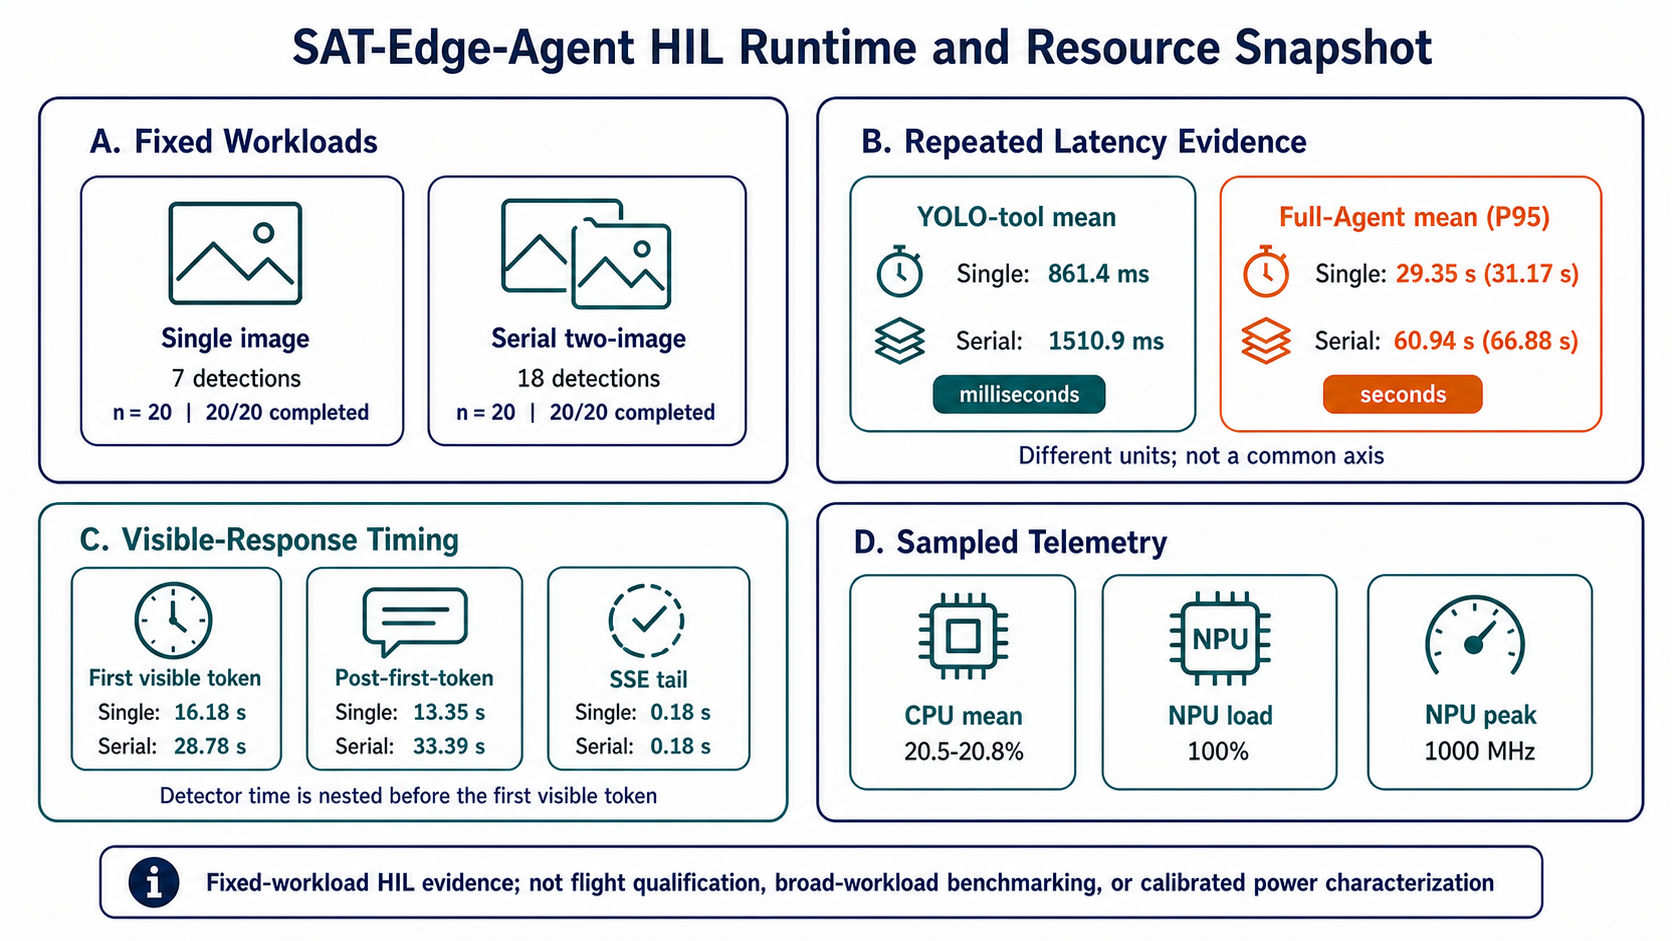
\includegraphics[width=0.98\textwidth]{figures/fig3_runtime_resource_snapshot.png}
\caption{Repeated HIL evidence for the two fixed FAIR1M workloads. Panel A defines the protocol. Panel B separates mean YOLO-tool latency in milliseconds from mean and empirical-P95 full-Agent latency in seconds; the cards do not encode a common axis. Panel C reports validated profiler intervals in seconds, with detector time identified as nested before the first visible response token rather than as an additive stage. Panel D reports the 200-ms sampled shared-accelerator NPU-load field and the $20.5$--$20.8\%$ range of the two per-workload mean CPU values. The separate 2026-07-03 plug-meter pilot is intentionally excluded.}
\label{fig:runtime_resource_snapshot}
\end{figure*}

\begin{table}[htbp]
\centering
\small
\renewcommand{\arraystretch}{1.12}
\setlength{\tabcolsep}{4pt}
\caption{Repeated full-Agent, YOLO-tool, and sampled resource statistics for the fixed FAIR1M workloads ($n=20$ each). Resource fields were sampled every 200 ms across the full request. CPU peak is the maximum observed per-request peak field, not a platform limit; the NPU field is not detector-only occupancy.}
\label{tab:agent_runtime_resource}
\begin{tabular}{p{0.43\linewidth}p{0.23\linewidth}p{0.23\linewidth}}
\toprule
\rowcolor{gray!12}
\textbf{Metric} & \textbf{Single image} & \textbf{Serial two-image} \\
\midrule
Observed completion & 20/20 & 20/20 \\
\rowcolor{graybg}
Full-Agent mean $\pm$ sample SD & $29.353 \pm 1.613$ s & $60.937 \pm 3.512$ s \\
Full-Agent median & 29.030 s & 61.134 s \\
\rowcolor{graybg}
Full-Agent empirical P95 & 31.166 s & 66.882 s \\
Full-Agent range & 26.919--34.504 s & 54.379--68.263 s \\
\rowcolor{graybg}
YOLO-tool mean $\pm$ sample SD & $861.386 \pm 11.778$ ms & $1510.920 \pm 18.180$ ms \\
YOLO-tool median & 863.415 ms & 1513.604 ms \\
\rowcolor{graybg}
YOLO-tool empirical P95 & 876.657 ms & 1535.151 ms \\
Detector share of mean Full-Agent latency & 2.93\% & 2.48\% \\
\rowcolor{graybg}
Mean sampled CPU utilization & 20.761\% & 20.482\% \\
Maximum observed CPU peak field & 86.335\% & 87.742\% \\
\rowcolor{graybg}
Mean 200-ms sampled NPU-load field & 100\% & 100\% \\
Peak sampled NPU frequency & 1000 MHz & 1000 MHz \\
\bottomrule
\end{tabular}
\end{table}

The repeated measurements show that detector execution is a small, workload-bounded fraction of the end-to-end request. It accounts for 2.93\% of the single-image mean and 2.48\% of the serial two-image mean. This finding does not imply that every remaining interval is pure language-model generation. The full-Agent window also includes Agent decisions, request construction, tool-result handling, annotated-output production, and response streaming. Likewise, the 100\% sampled NPU field does not imply continuous detector execution because the field covers shared accelerator activity over the complete request.

\subsection{Validated Visible-Response Timeline}

A separate profiler-enabled run set captures the event order \texttt{start} $\rightarrow$ \texttt{tool} $\rightarrow$ \texttt{token} $\rightarrow$ \texttt{done}. All 20 single-image profiler attempts completed. Nineteen serial two-image attempts completed both images; one additional attempt produced the structured 1/2 partial result described in the workflow section and is excluded from the all-images-successful timing mean. Table~\ref{tab:response_timeline} uses only fields validated against the raw SSE captures.

\begin{table}[htbp]
\centering
\small
\renewcommand{\arraystretch}{1.13}
\setlength{\tabcolsep}{4pt}
\caption{Mean response-timeline intervals for successful profiler-enabled runs. ``First visible token'' is an end-to-end user-visible boundary that includes pre-output Agent and tool activity; it is not pure LLM first-token latency. Detector time is nested inside that interval and must not be added to the other rows.}
\label{tab:response_timeline}
\begin{tabular}{p{0.43\linewidth}p{0.23\linewidth}p{0.23\linewidth}}
\toprule
\rowcolor{gray!12}
\textbf{Metric} & \textbf{Single image} & \textbf{Serial two-image} \\
\midrule
All-images-successful attempts & 20 & 19 \\
\rowcolor{graybg}
Full-Agent mean & 29.713 s & 62.362 s \\
Time to first visible response token & 16.184 s & 28.785 s \\
\rowcolor{graybg}
Post-first-token generation interval & 13.347 s & 33.392 s \\
SSE tail after final token & 0.182 s & 0.185 s \\
\rowcolor{graybg}
Detector-total mean (nested) & 0.857 s & 1.506 s \\
\bottomrule
\end{tabular}
\end{table}

The component CSV also contains batch HTTP, decode, inference, and annotation/render substage fields. Audit against all raw serial-batch captures found a systematic factor-of-two aggregation defect in those fields, so they are excluded from the manuscript. The validated timeline supports a narrower conclusion: most user-facing latency lies outside detector execution, both before and after the first visible token, and optimization should target the broader Agent and response-formation path.

\subsection{End-to-End Reproducibility Matrix}

Table~\ref{tab:repro_matrix} separates what a reader can reproduce directly from what remains private or replaceable. This distinction is important because the detector weight and private edge host are not the scientific contribution of the present paper.

\begin{table}[htbp]
\centering
\renewcommand{\arraystretch}{1.16}
\setlength{\tabcolsep}{4pt}
\caption{Reproducibility boundary for the SAT-Edge-Agent HIL system paper.}
\label{tab:repro_matrix}
\begin{tabular}{p{0.28\linewidth}p{0.28\linewidth}p{0.30\linewidth}}
\toprule
\rowcolor{gray!12}
\textbf{Layer} & \textbf{Publicly reproducible} & \textbf{Boundary or substitute path} \\
\midrule
Frontend/backend code & Build and run workflow, API routes, SSE stream contract & Private hostnames and paths are sanitized \\
\rowcolor{graybg}
Vision-tool contract & Health, model-status schema, success/failure JSON examples & Private YOLO weight can be replaced by a user-provided OBB model \\
Local LLM interface & OpenAI-compatible endpoint contract & Exact local model may be deployment-specific \\
\rowcolor{graybg}
Dataset sample & FAIR1M-style schema and license notes & FAIR1M-derived images must follow original dataset terms \\
Repeated timing evidence & Sanitized request-level CSVs, summary JSON/Markdown, recalculation script, and Figure 3 & Covers only the two declared fixed workloads \\
\rowcolor{graybg}
SSE and JSON contracts & Redacted success/failure JSON and normalized success/partial-result SSE examples & Raw identifiers, paths, base64 imagery, private labels, and operator text are omitted \\
Power evidence & Appendix-level plug-meter context and a public trace template & A synchronized calibrated trace is required before energy claims \\
\bottomrule
\end{tabular}
\end{table}

The reproducibility matrix separates public artifacts from replaceable or private components. The released package is located at \texttt{artifacts/hil\_orchestration/} and includes a SHA-256 manifest. Remaining workload-generalization, tail-latency, power, robustness, and metadata limitations are consolidated in the Limitations section and Appendix~\ref{app:artifacts} rather than repeated as a second evidence-gap table.


\section{Discussion}

\subsection{System Value of the Agent Layer}

The agent layer matters because it turns model endpoints into a task workflow. A detector endpoint alone returns boxes. An agent workflow can decide when to call the detector, stream tool state, summarize mission-relevant findings, and format outputs for humans or machines. This is the system gap that SAT-Edge-Agent addresses. The structured detector artifact remains the authoritative machine-facing result; natural-language synthesis is an optional operator-facing layer that can be shortened, deferred, or replaced without changing the detector contract. The measured narrative path, with mean first-visible-token boundaries of 16.184 s and 28.785 s, is not suitable for time-critical closed-loop control. In such paths, a downstream machine service should consume the structured tool event directly and treat language synthesis as a separable operator aid. This is an architectural interpretation of the observed event order, not a measured schema-only speedup claim.

\subsection{HIL and Measurement Boundary}

The HIL evidence is valuable because it grounds the architecture in a real edge-host runtime rather than only a diagram. The repeated experiment adds 20 completed attempts for each of two fixed FAIR1M workloads, a validated response-timeline decomposition, repeated CPU/NPU telemetry, and a structured 1/2 partial-batch case. The 100\% NPU-load field is a 200-ms devfreq/sysfs sample over a request window in which both local inference services can use the accelerator; it is not per-service occupancy and does not contradict the detector's 2--3\% share of end-to-end latency. The separate plug-meter pilot is likewise not synchronized with these runs and remains Appendix-level context. This evidence strengthens the paper from a point demonstration to a bounded repeatability study, but it remains workload-specific. HIL evidence is not a substitute for flight validation: radiation-aware design review, watchdog and recovery tests, thermal-vacuum or equivalent environmental testing, and a flight or RF-in-the-loop campaign remain necessary before any in-orbit claim is appropriate.

\subsection{Artifact and Release Boundary}

The public release provides sanitized request-level CSV files, redacted success and invalid-input JSON, normalized success and partial-failure SSE examples, a statistics script, and a SHA-256 manifest. The YOLO weight remains a non-public internal training asset, and the exact board and local language-model identities remain intentionally withheld. The term YOLO26 is retained only as a project-internal service/model label for the implemented YOLO-style OBB endpoint. Readers can replace the private detector and language service with compatible endpoints while preserving the documented contracts. FAIR1M-derived images remain governed by their original dataset license, not the repository software license, and are not redistributed in the public evidence package.

\section{Limitations}

The current manuscript is intentionally narrow in what it claims. \textbf{Deployment qualification.} The work reports a ground-based HIL edge deployment, not an in-orbit demonstration, radiation qualification, or flight-computer certification. \textbf{Perception and metadata.} YOLO26 is a project-internal label for a YOLO-style OBB tool; the paper does not report detector mAP, SOTA accuracy, training-protocol comparison, or independently validated geolocation error. Geographic fields are propagated from FAIR1M-style metadata rather than derived from a validated sensor model.

\textbf{Measurement scope.} The repeated evidence covers one fixed FAIR1M image and one fixed serial two-image pair, with 20 attempts per workload; it does not establish performance over a broader image, target-count, prompt, or concurrency distribution. Mean, sample SD, median, and empirical nearest-rank P95 are reported, but a robust P99 or general tail-latency claim is not supported by $n=20$. The first-visible-token interval includes Agent and tool activity and is not pure language-model first-token latency; frontend rendering and several internal orchestration substages remain unisolated. Power values come from a separate earlier plug-meter pilot, so calibrated traces, instrument metadata, sampling intervals, ambient temperature, and energy-per-request measurements are still required for a quantitative power study.

\textbf{Operational robustness and release constraints.} The evidence demonstrates a structured invalid-file response and one serial-batch 1/2 partial result that still reached \texttt{done}, but not comprehensive timeout, retry, watchdog, service-restart, or fault-recovery behavior. The public package exposes sanitized evidence and recalculation scripts, but the exact board identity, exact private language-model identity, detector weight, private runtime paths, and raw unredacted logs remain unavailable. FAIR1M-derived images remain governed by their original dataset license.

\section{Conclusion and Future Work}

SAT-Edge-Agent demonstrates an evidence-bounded HIL path toward satellite edge-agent orchestration. The system integrates a browser workspace, FastAPI agent backend, local LLM service, and YOLO-style OBB detector endpoint on a COTS ARM-based heterogeneous edge-SoC environment. For one fixed FAIR1M image and one fixed serial two-image pair, 20/20 attempts completed in each workload. Mean full-Agent latency was 29.353 s and 60.937 s, while detector execution represented 2.93\% and 2.48\% of those means. The evidence also verifies metadata-backed structured output, repeated CPU/NPU telemetry, visible-response timing, invalid-file handling, and a structured 1/2 partial-batch result. The strongest current claim remains architectural and systems-oriented: SAT-Edge-Agent shows how remote-sensing inference can be wrapped inside an observable onboard-style Agent workflow without presenting the detector, LLM, geographic metadata, or power observations as standalone algorithmic or flight-qualified results.

Future work should broaden the workload distribution, evaluate concurrency and larger image batches, instrument finer orchestration and frontend stages, and collect enough runs for defensible tail-latency analysis. A controlled schema-only versus narrative-enabled experiment is also needed before quantifying the latency benefit of deferring natural-language synthesis. Calibrated watt-level power and energy measurements, watchdog and fault-injection tests, and an RF or flight-like environmental validation path remain separate requirements for a more complete onboard edge-agent systems study.

The agent code, model/runtime card, dataset-license notes, sanitized evidence package, representative JSON and SSE outputs, power-measurement trace template, and reproducibility instructions will be released with the public arXiv package at \url{https://github.com/keithhegit/SAT-Edge-Agent}. Private hostnames, IP addresses, VM access details, hardware vendor-sensitive labels, exact private model identities, and internal deployment paths remain replaced by placeholders such as \texttt{<edge-host>}. Appendix~\ref{app:artifacts} summarizes the artifact inventory and release boundary.

\clearpage
\appendix
\renewcommand{\thesection}{Appendix \Alph{section}}

\section{Reproducibility and Release Boundary}
\label{app:artifacts}

This appendix records the public evidence, measurement definitions, and release boundary used by the current SAT-Edge-Agent manuscript. Repository paths are relative to the public project root.

\subsection{Public Artifact Inventory}

\begin{table}[H]
\centering
\footnotesize
\renewcommand{\arraystretch}{1.15}
\setlength{\tabcolsep}{4pt}
\caption{Public artifacts supporting the HIL orchestration claims.}
\label{tab:hil_artifacts}
\begin{tabular}{p{0.34\linewidth}p{0.53\linewidth}}
\toprule
\rowcolor{gray!12}
\textbf{Artifact} & \textbf{Repository path} \\
\midrule
Public evidence guide & \texttt{artifacts/hil\_orchestration/README.md} \\
\rowcolor{graybg}
Repeated fixed-workload rows & \texttt{artifacts/hil\_orchestration/data/}
\newline\texttt{fixed\_workload\_runs.csv} \\
Visible-response profiler rows & \texttt{artifacts/hil\_orchestration/data/}
\newline\texttt{visible\_response\_timing.csv} \\
\rowcolor{graybg}
Derived result summaries & \texttt{artifacts/hil\_orchestration/results/}
\newline\texttt{hil\_orchestration\_summary.json}, \texttt{hil\_orchestration\_summary.md} \\
Recalculation script & \texttt{artifacts/hil\_orchestration/scripts/}
\newline\texttt{summarize\_public\_metrics.py} \\
\rowcolor{graybg}
Redacted API examples & \texttt{artifacts/hil\_orchestration/examples/}
\newline\texttt{detect\_success\_redacted.json}, \texttt{detect\_failure\_redacted.json} \\
Normalized SSE examples & \texttt{artifacts/hil\_orchestration/examples/}
\newline\texttt{sse\_success\_normalized.jsonl},
\newline\texttt{sse\_partial\_failure\_normalized.jsonl} \\
\rowcolor{graybg}
Integrity manifest & \texttt{artifacts/hil\_orchestration/MANIFEST.sha256} \\
Model/runtime and reproduction boundary & \texttt{MODEL\_CARD.md}, \texttt{REPRODUCIBILITY.md} \\
\rowcolor{graybg}
Dataset acquisition and checksums & \texttt{dataset/README.md}, \texttt{dataset/DATA\_LICENSE.md},
\newline\texttt{dataset/sample\_100\_mix\_manifest.csv},
\newline\texttt{dataset/sample\_100\_mix\_sha256.csv} \\
Power-trace field template & \texttt{artifacts/hil\_orchestration/templates/}
\newline\texttt{power\_trace\_template.csv} \\
\bottomrule
\end{tabular}
\end{table}

The public CSV rows are field-level redactions of the internal request records. They remove source-capture names, timestamps, request and thread identifiers, input paths, exact private model labels, and operator text. Running the public script recalculates the means, sample standard deviations, medians, nearest-rank empirical P95 values, detector shares, and profiler means reported in the manuscript.

\subsection{Normalized Service Examples}

The normalized success transcript preserves the event order and selected validated values while omitting payload imagery and natural-language content:

\begin{small}
\begin{verbatim}
event: start
event: tool  {"phase":"result","success_count":1,
              "failure_count":0,"total_detections_count":7}
event: token {"text":"<operator-facing summary omitted>"}
event: done  {"duration_ms":29722,
              "detector_total_ms":851.794,
              "time_to_first_visible_token_ms":19966}
\end{verbatim}
\end{small}

The partial-result example records two requested inputs, one successful input, one unavailable input, seven retained detections, a final operator-facing response, and the terminal \texttt{done} event:

\begin{small}
\begin{verbatim}
event: start
event: tool  {"phase":"result","success_count":1,
              "failure_count":1,"total_detections_count":7}
event: token {"text":"<partial-result summary omitted>"}
event: done  {"duration_ms":57300,
              "completion_status":"partial_result"}
\end{verbatim}
\end{small}

These examples support event-contract and structured-degradation claims. They do not establish retry, timeout recovery, watchdog behavior, or service restart correctness.

\subsection{Telemetry and Power Boundaries}

CPU counters and the NPU devfreq/sysfs load/frequency field were sampled every 200 ms across the complete Full-Agent request. The detector and local language service can both use the accelerator. The reported 100\% mean NPU-load field is therefore a coarse shared-accelerator software value rather than detector-only occupancy, per-service attribution, or calibrated utilization.

Power observations were collected in a separate 2026-07-03 pilot with different workloads. They are retained as board-level HIL context but are not synchronized with the repeated FAIR1M measurements. The manuscript therefore does not derive energy per request by multiplying the following observations by the 2026-07-13 latency statistics.

\begin{table}[H]
\centering
\renewcommand{\arraystretch}{1.14}
\setlength{\tabcolsep}{4pt}
\caption{Board-level plug-meter observations from the separate pilot. These values do not constitute a calibrated continuous spacecraft power trace.}
\label{tab:power_snapshot}
\begin{tabular}{p{0.24\linewidth}p{0.18\linewidth}p{0.43\linewidth}}
\toprule
\rowcolor{gray!12}
\textbf{Operating state} & \textbf{Observed power} & \textbf{Evidence boundary} \\
\midrule
Idle baseline & $\sim$3 W & Manual plug-meter screen observation before request and after recovery \\
\rowcolor{graybg}
Active-load interval & $\sim$8--9 W & Manual observation during detection and local Agent response formation \\
Post-output transition & $\sim$4 W & Manual observation after output and before idle recovery \\
\bottomrule
\end{tabular}
\end{table}

The public trace template declares the fields needed for a stronger study: timestamp, workload state, voltage, current, power, board temperature, ambient temperature, and note. A calibrated instrument description, measured rail, sampling period, timestamp alignment, and synchronized workload script remain necessary before reporting peak power, energy per request, or thermal behavior.

\subsection{Data, Model, and Privacy Boundary}

FAIR1M-derived images, labels, and geographic fields are third-party data governed by the original FAIR1M/Kaggle terms. The repository publishes source attribution, download instructions, a 100-file manifest, image checksums, and a narrowly redacted output example, but not the image files or full internal metadata bundle. FAIR1M-derived fields in the example remain subject to the source data terms rather than the repository software license. The detector weight is an internal training asset and is not redistributed. The exact board model, exact private language-model identity, private generation throughput, hostnames, IP addresses, VM access methods, internal paths, and raw unredacted logs are also withheld.

The public reproduction path is contract-based. Readers may use a compatible OBB endpoint and an OpenAI-compatible local language endpoint, or recalculate the manuscript statistics directly from the released sanitized evidence. The earlier Qwen Instruct 16K capability benchmark remains separate supplementary material and is not identified as the exact configuration used by the 2026-07-13 repeated HIL experiment.

\subsection{Claim Boundary}

The current manuscript does not claim flight validation, radiation qualification, detector SOTA accuracy, complete model-weight reproduction, independently validated geolocation error, broad-workload latency generalization, robust P99 latency, calibrated power or energy characterization, or a complete autonomous mission scheduler. Each stronger claim would require evidence beyond the fixed-workload HIL measurements, public service examples, runtime profile, and separate plug-meter pilot reported here.

\clearpage

\clearpage

\begin{thebibliography}{99}

\bibitem{phisat1}
G. Giuffrida \emph{et al.}, The Phi-Sat-1 Mission: The First On-Board Deep Neural Network Demonstrator for Satellite Earth Observation, \emph{IEEE Transactions on Geoscience and Remote Sensing}, 2022, doi: 10.1109/TGRS.2021.3125567.

\bibitem{eo1_sciencecraft}
S. Chien \emph{et al.}, The Autonomous Sciencecraft Experiment, in \emph{Proceedings of the IEEE Aerospace Conference}, 2003, doi: 10.1109/AERO.2003.1235068.

\bibitem{onboard_classifiers}
R. Castano \emph{et al.}, Onboard Classifiers for Science Event Detection on a Remote Sensing Spacecraft, in \emph{Proceedings of the 12th ACM SIGKDD International Conference on Knowledge Discovery and Data Mining}, 2006, pp. 845-851, doi: 10.1145/1150402.1150519.

\bibitem{cloudscout}
G. Giuffrida \emph{et al.}, CloudScout: A Deep Neural Network for On-Board Cloud Detection on Hyperspectral Images, \emph{Remote Sensing}, vol. 12, no. 14, art. 2205, 2020, doi: 10.3390/rs12142205.

\bibitem{ravaen}
V. Ruzicka \emph{et al.}, RaVAEn: Unsupervised Change Detection of Extreme Events Using ML On-Board Satellites, \emph{Scientific Reports}, vol. 12, art. 16939, 2022, doi: 10.1038/s41598-022-19437-5.

\bibitem{fast_onboard_training}
V. Ruzicka \emph{et al.}, Fast Model Inference and Training On-Board of Satellites, arXiv:2307.08700, 2023.

\bibitem{oec_asplos}
B. Denby and B. Lucia, Orbital Edge Computing: Nanosatellite Constellations as a New Class of Computer System, in \emph{Proceedings of ASPLOS}, 2020, doi: 10.1145/3373376.3378473.

\bibitem{satedge_tcom}
I. Leyva-Mayorga, M. Martinez-Gost, M. Moretti, A. Perez-Neira, M. A. Vazquez, P. Popovski, and B. Soret, Satellite Edge Computing for Real-Time and Very-High Resolution Earth Observation, \emph{IEEE Transactions on Communications}, vol. 71, no. 10, pp. 6180-6194, 2023, doi: 10.1109/TCOMM.2023.3296584.

\bibitem{satellite_edge_large_models}
Y. Shi, J. Zhu, C. Jiang, L. Kuang, and K. B. Letaief, Satellite Edge Artificial Intelligence with Large Models: Architectures and Technologies, arXiv:2504.01676, 2025.

\bibitem{ai_onboard_survey}
A. Duggan, B. Andrade, and H. Afli, Advancing Earth Observation: A Survey on AI-Powered Image Processing in Satellites, arXiv:2501.12030, 2025.

\bibitem{gardill_space_edge}
M. Gardill \emph{et al.}, Towards Space Edge Computing and Onboard AI for Real-Time Teleoperations, IEEE Future Directions Low-Earth Orbit Satellites and Systems Initiative report, 2023.

\bibitem{edge_processor_benchmark}
E. R. Dunkel \emph{et al.}, Benchmarking Deep Learning Models on Myriad and Snapdragon Processors for Space Applications, \emph{Journal of Aerospace Information Systems}, vol. 20, no. 10, pp. 660-674, 2023, doi: 10.2514/1.I011216.

\bibitem{edge_ai_platform_benchmark}
R. Jayanth, N. Gupta, and V. Prasanna, Benchmarking Edge AI Platforms for High-Performance ML Inference, arXiv:2409.14803, 2024, doi: 10.48550/arXiv.2409.14803.

\bibitem{react}
S. Yao \emph{et al.}, ReAct: Synergizing Reasoning and Acting in Language Models, arXiv:2210.03629, 2022.

\bibitem{toolformer}
T. Schick \emph{et al.}, Toolformer: Language Models Can Teach Themselves to Use Tools, arXiv:2302.04761, 2023.

\bibitem{llm_agents_survey}
L. Wang \emph{et al.}, A Survey on Large Language Model Based Autonomous Agents, \emph{Frontiers of Computer Science}, vol. 18, art. 186345, 2024, doi: 10.1007/s11704-024-40231-1.

\bibitem{onboard_multiagent_eo}
A. D. Mousist, P. Delgado de Robles Mart\'{i}n, R. Lladr\'{o} Climent, and J. Cobos Aparicio, Beyond Detection: Cooperative Multi-Agent Reasoning for Rapid Onboard EO Crisis Response, arXiv:2603.19858, 2026, doi: 10.48550/arXiv.2603.19858.

\bibitem{dota}
G.-S. Xia \emph{et al.}, DOTA: A Large-Scale Dataset for Object Detection in Aerial Images, in \emph{Proceedings of the IEEE Conference on Computer Vision and Pattern Recognition}, 2018, doi: 10.1109/CVPR.2018.00418.

\bibitem{fair1m}
X. Sun \emph{et al.}, FAIR1M: A Benchmark Dataset for Fine-Grained Object Recognition in High-Resolution Remote Sensing Imagery, \emph{ISPRS Journal of Photogrammetry and Remote Sensing}, vol. 184, pp. 116-130, 2022, doi: 10.1016/j.isprsjprs.2021.12.004.

\bibitem{rsod_review}
S. Gui, S. Song, R. Qin, and Y. Tang, Remote Sensing Object Detection in the Deep Learning Era: A Review, \emph{Remote Sensing}, vol. 16, no. 2, art. 327, 2024, doi: 10.3390/rs16020327.

\bibitem{obb_survey}
K. Wang \emph{et al.}, Oriented Object Detection in Optical Remote Sensing Images Using Deep Learning: A Survey, \emph{Artificial Intelligence Review}, 2025, doi: 10.1007/s10462-025-11256-0.

\end{thebibliography}

\end{document}
